% Filtros dirigibles (steerable filters) y su descomposición
% Compilar con: pdflatex steerable_filters.tex
\documentclass[tikz,border=10pt]{standalone}
\usepackage{tikz}
\usepackage{amsmath,amssymb}
\usetikzlibrary{arrows.meta, positioning, calc, shadings, decorations.pathreplacing}

\definecolor{gdlblue}{RGB}{41, 98, 168}
\definecolor{gdlred}{RGB}{191, 49, 49}
\definecolor{gdlgreen}{RGB}{30, 130, 76}
\definecolor{gdlorange}{RGB}{217, 130, 30}
\definecolor{gdlpurple}{RGB}{118, 56, 138}
\definecolor{gdlgray}{RGB}{140, 140, 140}
\definecolor{gdlyellow}{RGB}{190, 140, 10}

% Command to draw a steerable filter (oriented edge detector) at a given angle
% #1 = center x, #2 = center y, #3 = rotation angle, #4 = radius
\newcommand{\steerablefilter}[4]{%
    \begin{scope}[shift={(#1,#2)}, rotate=#3]
        % White half (positive lobe)
        \fill[white, draw=gdlblue!60, thick] (0,0) -- (90:#4) arc (90:270:#4) -- cycle;
        % Blue half (negative lobe)
        \fill[gdlblue!30, draw=gdlblue!60, thick] (0,0) -- (270:#4) arc (270:450:#4) -- cycle;
        % Outer circle border (full)
        \draw[gdlblue!60, thick] (0,0) circle (#4);
        % Center line
        \draw[gdlgray!50, thin] (0,-#4) -- (0,#4);
    \end{scope}
}

% Command to draw a filter with a specific border color
% #1 = center x, #2 = center y, #3 = rotation angle, #4 = radius, #5 = border color
\newcommand{\steerablefiltercolor}[5]{%
    \begin{scope}[shift={(#1,#2)}, rotate=#3]
        % White half (positive lobe)
        \fill[white, draw=#5, thick] (0,0) -- (90:#4) arc (90:270:#4) -- cycle;
        % Colored half (negative lobe)
        \fill[gdlblue!30, draw=#5, thick] (0,0) -- (270:#4) arc (270:450:#4) -- cycle;
        % Outer circle border (full)
        \draw[#5, thick] (0,0) circle (#4);
        % Center line
        \draw[gdlgray!50, thin] (0,-#4) -- (0,#4);
    \end{scope}
}

\begin{document}
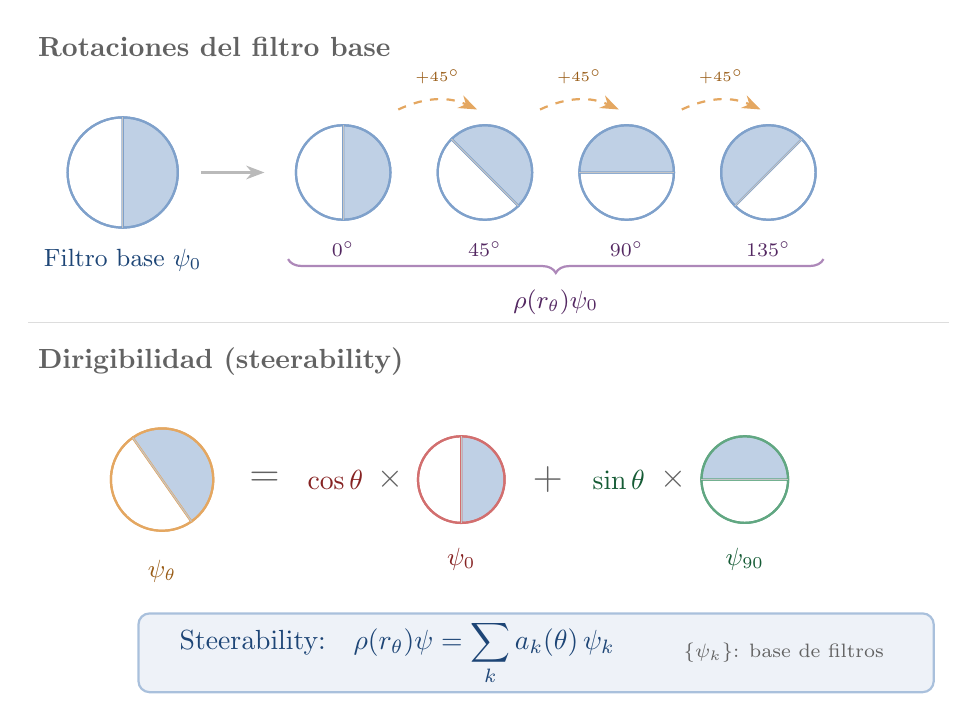
\begin{tikzpicture}[
    >=Stealth,
    every node/.style={font=\small},
    section label/.style={font=\normalsize\bfseries, text=gdlgray!70!black}
]

% =============================================
% TOP ROW: Base filter and rotated versions
% =============================================

% Section label
\node[section label, anchor=west] at (-1.2, 2.8) {Rotaciones del filtro base};

% Base filter (0 degrees)
\steerablefilter{0}{1.2}{0}{0.7}
\node[below, text=gdlblue!70!black, font=\small] at (0, 0.35)
    {Filtro base $\psi_0$};

% Arrow from base to rotated versions
\draw[->, thick, gdlgray!60] (1.0, 1.2) -- (1.8, 1.2);

% Rotated at 0 degrees
\steerablefilter{2.8}{1.2}{0}{0.6}
\node[below, text=gdlpurple!70!black, font=\scriptsize] at (2.8, 0.45)
    {$0^\circ$};

% Rotated at 45 degrees
\steerablefilter{4.6}{1.2}{45}{0.6}
\node[below, text=gdlpurple!70!black, font=\scriptsize] at (4.6, 0.45)
    {$45^\circ$};

% Rotated at 90 degrees
\steerablefilter{6.4}{1.2}{90}{0.6}
\node[below, text=gdlpurple!70!black, font=\scriptsize] at (6.4, 0.45)
    {$90^\circ$};

% Rotated at 135 degrees
\steerablefilter{8.2}{1.2}{135}{0.6}
\node[below, text=gdlpurple!70!black, font=\scriptsize] at (8.2, 0.45)
    {$135^\circ$};

% Decorative brace below angle labels
\draw[gdlpurple!60, thick, decorate, decoration={brace, amplitude=5pt, mirror}]
    (2.1, 0.1) -- (8.9, 0.1);
\node[below=6pt, text=gdlpurple!70!black, font=\small] at (5.5, 0.05)
    {$\rho(r_\theta)\psi_0$};

% Curved rotation arrows between adjacent filters
\draw[->, gdlorange!70, thick, dashed]
    (3.5, 2.0) to[bend left=25] (4.5, 2.0);
\draw[->, gdlorange!70, thick, dashed]
    (5.3, 2.0) to[bend left=25] (6.3, 2.0);
\draw[->, gdlorange!70, thick, dashed]
    (7.1, 2.0) to[bend left=25] (8.1, 2.0);

% Small rotation angle labels above arrows
\node[above, font=\tiny, text=gdlorange!70!black] at (4.0, 2.2) {$+45^\circ$};
\node[above, font=\tiny, text=gdlorange!70!black] at (5.8, 2.2) {$+45^\circ$};
\node[above, font=\tiny, text=gdlorange!70!black] at (7.6, 2.2) {$+45^\circ$};

% =============================================
% BOTTOM: Steerability equation (visual)
% =============================================

% Separator line
\draw[gdlgray!30, thin] (-1.2, -0.7) -- (10.5, -0.7);

% Section label
\node[section label, anchor=west] at (-1.2, -1.2) {Dirigibilidad (steerability)};

% The equation: ψ_θ = cos θ · ψ_0 + sin θ · ψ_90
% Left side: rotated filter at angle θ
\steerablefiltercolor{0.5}{-2.7}{35}{0.65}{gdlorange!70}
\node[below, text=gdlorange!70!black, font=\small] at (0.5, -3.6)
    {$\psi_\theta$};

% Equals sign
\node[font=\Large, text=gdlgray!70!black] at (1.8, -2.7) {$=$};

% cos θ coefficient
\node[font=\normalsize, text=gdlred!70!black] at (2.7, -2.7) {$\cos\theta$};

% Multiplication sign
\node[font=\large, text=gdlgray!70!black] at (3.4, -2.7) {$\times$};

% Horizontal basis filter (ψ_0)
\steerablefiltercolor{4.3}{-2.7}{0}{0.55}{gdlred!70}
\node[below, text=gdlred!70!black, font=\small] at (4.3, -3.45)
    {$\psi_0$};

% Plus sign
\node[font=\Large, text=gdlgray!70!black] at (5.4, -2.7) {$+$};

% sin θ coefficient
\node[font=\normalsize, text=gdlgreen!70!black] at (6.3, -2.7) {$\sin\theta$};

% Multiplication sign
\node[font=\large, text=gdlgray!70!black] at (7.0, -2.7) {$\times$};

% Vertical basis filter (ψ_90)
\steerablefiltercolor{7.9}{-2.7}{90}{0.55}{gdlgreen!70}
\node[below, text=gdlgreen!70!black, font=\small] at (7.9, -3.45)
    {$\psi_{90}$};

% =============================================
% General steerability formula (boxed)
% =============================================

% Background box
\fill[gdlblue!8, rounded corners=4pt]
    (0.2, -4.4) rectangle (10.3, -5.4);
\draw[gdlblue!40, rounded corners=4pt, thick]
    (0.2, -4.4) rectangle (10.3, -5.4);

% General formula
\node[font=\normalsize, text=gdlblue!70!black, anchor=west] at (0.6, -4.9)
    {Steerability:\quad $\displaystyle \rho(r_\theta)\psi
     = \sum_{k} a_k(\theta)\,\psi_k$};

% Annotation for basis
\node[font=\scriptsize, text=gdlgray!70!black, anchor=west] at (7.0, -4.9)
    {$\{\psi_k\}$: base de filtros};

\end{tikzpicture}
\end{document}
